
\vspace{-1.3\baselineskip}
\section{Introduction}
\vspace{-0.5\baselineskip}
\label{sec:introduction}
% the problem we are solving, distinguish with previous problems
In applications like robotic navigation~\cite{ohno2003outdoor} or augment reality~\cite{DBLP:journals/corr/abs-1708-05006}, visual-based 6-DOF camera pose estimation~\cite{campbell2017globally,moreno2008pose,Kendall_2015_ICCV,coskun2017long}, and concurrently parsing each frame of a video into semantically meaningful regions~\cite{ZhaoSQWJ16,WuSH16e,ChenPSA17} efficiently are the key components, which are attracting much attention in computer vision.
% Additionally, to acquire better scene understanding for , is also important.

\begin{figure*}[t]
\center
\vspace{-1\baselineskip}
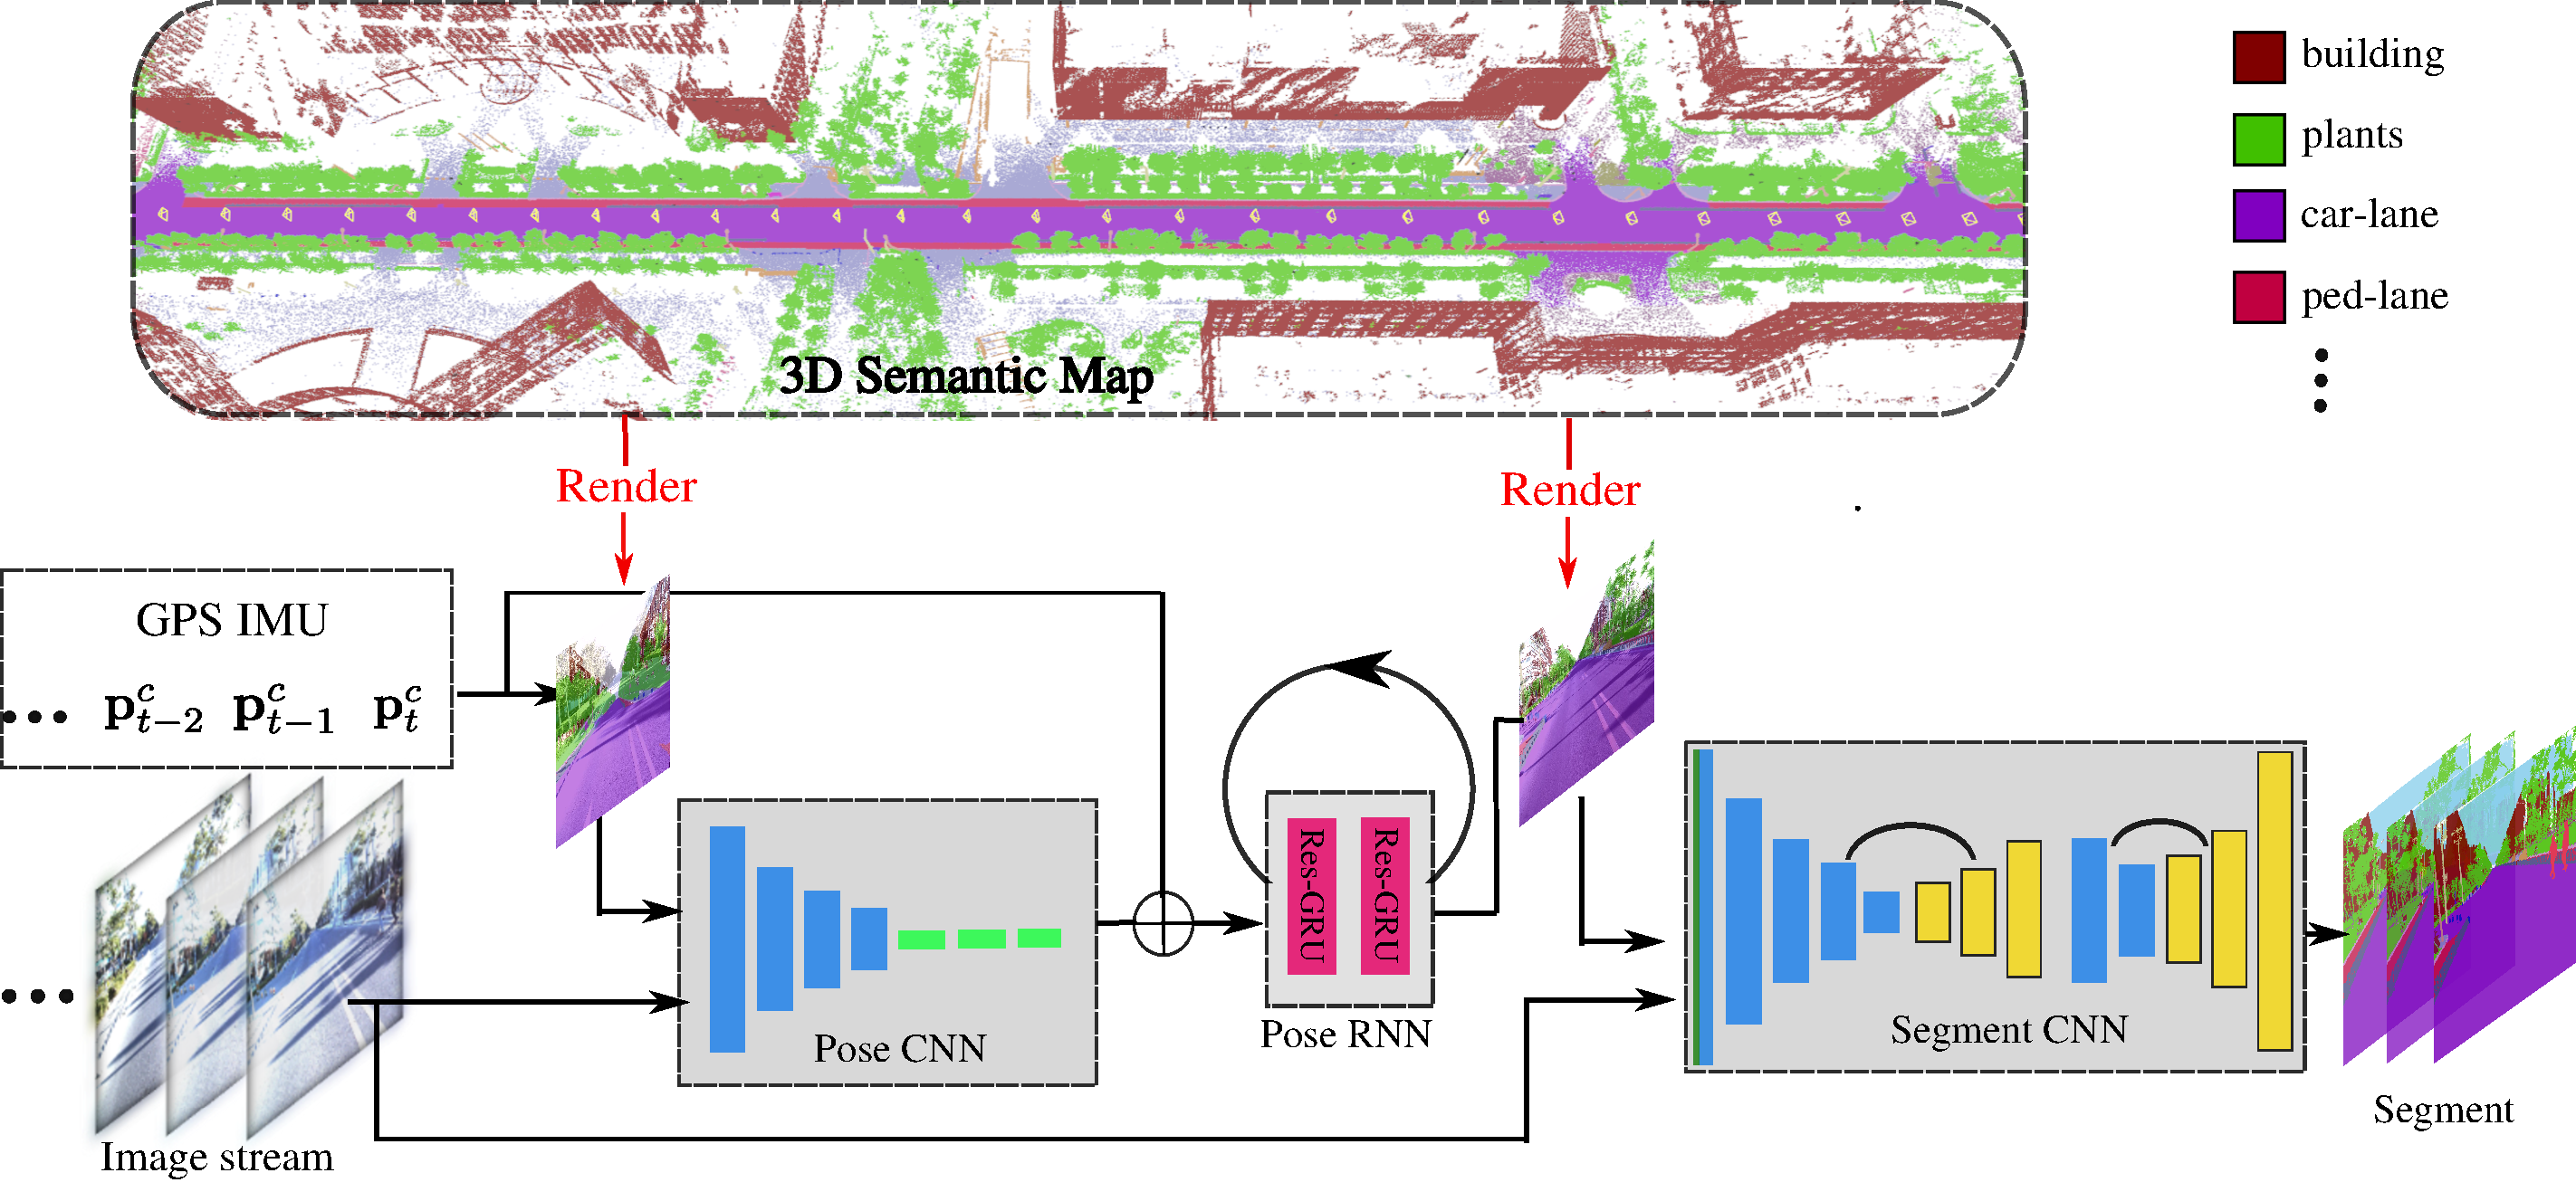
\includegraphics[width=0.9\textwidth]{fig/framework.pdf}
\caption{System overview. The black arrows show the testing process, and red arrows indicate the rendering (projection) operation in training and inference. The yellow frustum shows the location of cameras inside the 3D map. The input of our system contains a sequence of images and corresponding GPS/IMU signals. The outputs are the semantically segmented images, each with its refined camera pose.}
\label{fig:framework}
\vspace{-1\baselineskip}
\end{figure*}

% existing methods only consider one of the tasks with soly visual signal.
Currently, most state-of-the-art (SOTA) algorithms try to solve both tasks using solely visual signals.
For camera localization, geometric based methods are relying on visual feature matching, \eg~systems of Perspective-n-Points (PnP)~\cite{haralick1994review,kneip2014upnp,campbell2017globally} when a 3D map and an image is provided, or systems of SLAM~\cite{engel2014lsd,mur2015orb,NewcombeLD11} when there is a video. Such systems are dependent on local appearance, which could fail when confronted with low-texture environments.
Most recently, deep learning based methods, \eg~for either images~\cite{Kendall_2015_ICCV} or videos~\cite{DBLP:journals/corr/ClarkWMTW17}, have been developed, which not only consider hierarchical features, while yielding real-time performance. %which show good trade-offs between accuracy and speed.
Nevertheless, those methods are good for environments with rich distinguishable features, such as these in the Cambridge landmarks dataset~\cite{Kendall_2015_ICCV}. They could fail for common street views with very similar appearances or even repetitive structures.
%For example, when driving inside a tree-line street beside, can hardly localize the images without external signals.

For scene parsing, approaches~\cite{ZhaoSQWJ16,ChenPSA17} based on deep fully convolutional network (FCN) with ResNet~\cite{HeZRS15} are the best-performing algorithms for single image input. When the input is video, researchers~\cite{kundu2016feature,zhu2016deep} incorporate the optical flow between consecutive frames, which not only accelerates the parsing, but also improve temporal consistency. Furthermore, for static background, one may use structure-from-motion (SFM) techniques~\cite{wu2011visualsfm} to jointly parse and reconstruct~\cite{kundu2014joint}. However, these methods could be either time-consuming or hard to generalize for applications asking online real-time performance.

In this paper, we aim to solve this camera localization and scene parsing problem jointly from a more practical standpoint. In our system, we assume to have (a) GPS/IMU signal to provide a coarse camera pose estimation; (b) a semantic 3D map for the static environment. The GPS/IMU signals serve as a crucial prior for our deep-learning based pose estimation system. The semantic 3D map, which can synthesize a semantic view for a given camera pose, not only provides strong guidance for scene parsing, but also helps maintain temporal consistency.
%In our scenario, targeting at a more practical setting, we consider the video is online recorded, and a 3D semantic map is pre-built by us. For handling the localization confusion of street views, we propose to fuse signals from motion sensors like global positioning system (GPS) and inertial measurement unit (IMU), which is typically available for current navigation system. Those signals can be noisy but is crucial as a pose priori for our deep learning system.
%For video segmentation, we online render images from the 3D map, which serves as a priori for further segmentation, and helps the consistency along the temporal dimension.
%
Our setting is considered on par with the widely used mobile navigation systems, whereas the 2D labeled map is replaced with a 3D semantic map, and we are able to virtually place the navigation signals into the images with more accurate self-localization and scene parsing on-the-fly. 
Promisingly, with the accelerated development of autonomous driving, city-scale 3D semantic maps are being collected and built (such as the TorontoCity dataset~\cite{wang2016torontocity}). Here, we constructed our own data with high quality 3D semantic map, which is captured via a high-accuracy mobile LIDAR device from $Riegl$\footnote{http://www.rieglusa.com/index.html}.

%lots of city scale 3D map has already collected from companies such as Google Earth~\cite{sheppard2009ethics} and Altizure\footnote{https://www.altizure.com/}, and also semantic labeled ones is also built such as Toronto city~\cite{wang2016torontocity}. In our case, we constructed our own data with high quality 3D semantic map, by adopting a high accuracy mobile LIDAR device from Riegl\footnote{http://www.rieglusa.com/index.html}.
Last but not least, within our deep learning framework, the camera poses and scene semantics are mutually beneficial. The camera poses help establish the correspondences between the 3D semantic map and 2D semantic label map. Conversely, scene semantics could help refine camera poses. Our unified framework yields better results, in terms of both accuracy and speed, for both tasks than doing them individually. In our experiments, using a single Titan Z GPU, the networks in our system estimates the pose in 10ms with accuracy under 1 degree, and segments the image $512 \times 608$ in within 90ms with pixel accuracy around 96$\%$ without model compression, which demonstrates its efficiency and effectiveness.

% redefine our problem
In summary, the contributions of this paper are:
\begin{itemize}
\vspace{-0.5\baselineskip}
    \setlength{\itemsep}{-2pt}
    \item We propose a deep learning based system for fusing multiple sensors, \ie~RGB images, customer-grad GPS/IMU, and 3D semantic maps, which improves the robustness and accuracy for camera localization and scene parsing.
    \item Camera poses and scene semantics are designed to handle jointly in a unified framework.
    \item We create a dataset from real scenes to fully evaluate our approach. It includes dense 3D semantically labelled point clouds, ground truth camera poses and pixel-level semantic labels of video camera images, which will be released in order to benefit related researches.
\vspace{-0.4\baselineskip}
\end{itemize}

The structure of this paper is organized as follows. We first give an overview of our system in \secref{sub:framework} and talk about related works in \secref{sec:related_work}. In \secref{sec:data_collection}, we describe the uniqueness of our data from the existing outdoor datasets, and introduce our collection and labelling process. 
Then, \secref{sec:localize_and_parsing} presents details of our system. We perform full evaluation quantitatively for both pose estimation and scene parsing in \secref{sec:experiments}, and \secref{sec:conclusion} concludes the paper and points out future directions. % Finally, we will release our code, models and dataset with the publication of this paper.

\vspace{-0.7\baselineskip}
\subsection{Framework}
\vspace{-0.6\baselineskip}
\label{sub:framework}
The framework of our system is illustrated in \figref{fig:framework}. At upper part, a pre-built 3D semantic map is available. During testing, an online stream of images and corresponding coarse camera poses from GPS/IMU are fed into the system. Firstly, for each frame, a semantic label map is rendered out given the input coarse camera pose, which is fed into a pose CNN jointly with the respective RGB image.  The network calculates the relative rotation and translation, and yields a corrected camera pose. To incorporate the temporal correlations, the corrected poses from pose CNN are fed into a pose RNN to further improves the estimation accuracy in the stream.
Last, given the rectified camera pose, a new label map is rendered out, which is fed together with the image to a segment CNN. The rendered label map helps to segment a spatially more accurate and temporally more consistent result for the image stream of video.
In this system, since our data contains ground truth for both camera poses and segments, it can be trained with strong supervision at each end of outputs.
